%---------------------------------------------------------------------------------------------------
% file EPR.tex
%---------------------------------------------------------------------------------------------------
% !TeX spellcheck = cs_CZ
%================= Kapitola: TEORIE SPÍNACÍHO OBLOUKU===============================================
\setchaptertoc
\chapter{Teorie elektrického oblouku}
\section{Teorie spínacího oblouku}
  \subsection{Plazma elektrického oblouku}
    Ve spínací technice se zabýváme plazmatem vznikajícím hořením elektrického oblou\-ku při spínání
    elektrických obvodů. Dále popisované vlastnosti elektrického oblouku jsou rozpracovány pro druh
    plazmatu hořící ve vypínací dráze zhášecích komor vypínačů. Toto plazma se charakterizuje jako
    vysokotlaké (tlaky plynu vyšší než \qty{0.1}{\MPa}) a elektrické proudy řádově kilo-ampéry.
    Pozornost bude soustředěna zejména na elektrický oblouk hořící v tlakoplynových zhášecích
    komorách při vypínání elektrických obvodů. V tlakoplynových zhášecích komorách byl oblouk
    nejvíce prozkoumán u tlakovzdušného principu a u vypínačů s plynem \ce{SF6}
    \cite[s.~3]{BartaVostracky}.
  \subsection{Charakteristika vypínacího pochodu}
    \subsubsection{Základní uspořádání zhášecích komor}
      Základním uspořádání zhášecích komor lze rozdělit z hlediska proudění plynu na zhášecí komory:
      \begin{itemize}[noitemsep]
        \item s jednostranným prouděním,
        \item s dvoustranným prouděním.
      \end{itemize}

      \begin{figure}[ht!]
        \centering
        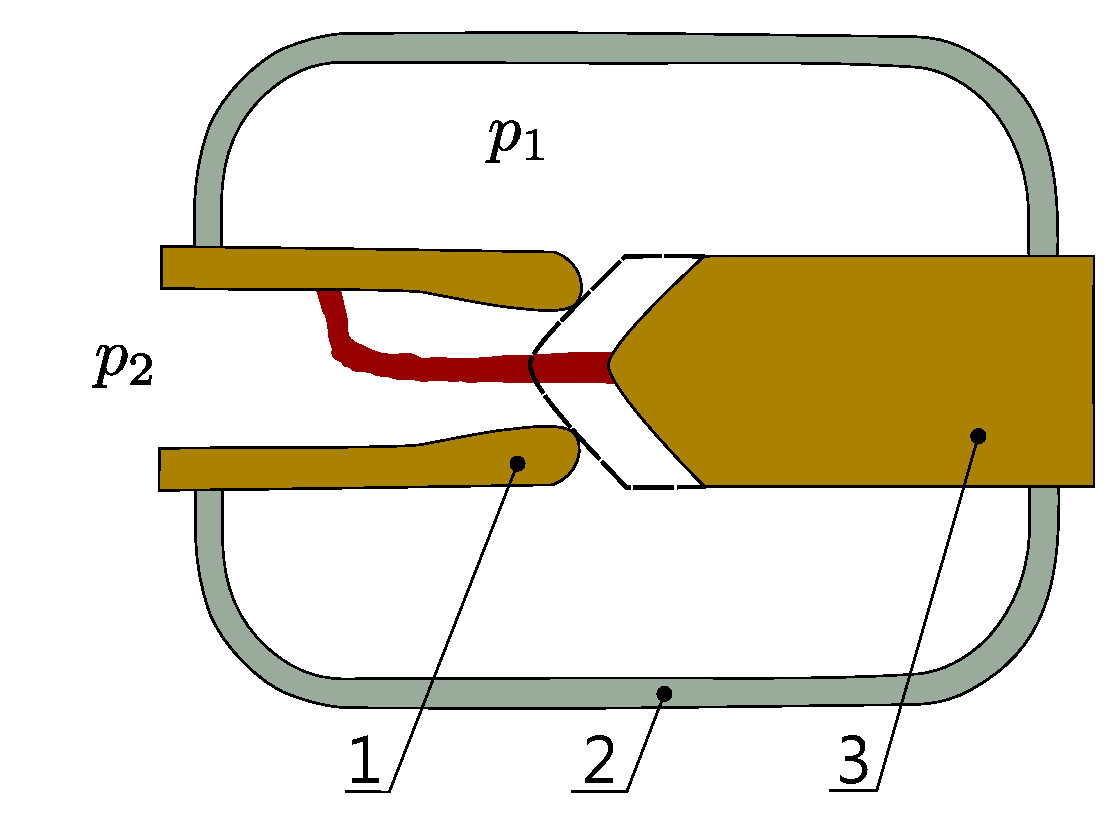
\includegraphics[width=0.6\linewidth]{Barta_Vostracky_Komora_jednostrannym_proudenim.pdf}
        \caption[Schématické uspořádání zhášecí komory tlakovzdušného vypínače s jednostranným
                 prouděním.]{Schématické uspořádání zhášecí komory tlakovzdušného vypínače s
                 jednostranným prouděním.}
        \label{epr:fig_komora_1stran_proudenim}
      \end{figure}

      \begin{figure}[ht!]
        \centering
        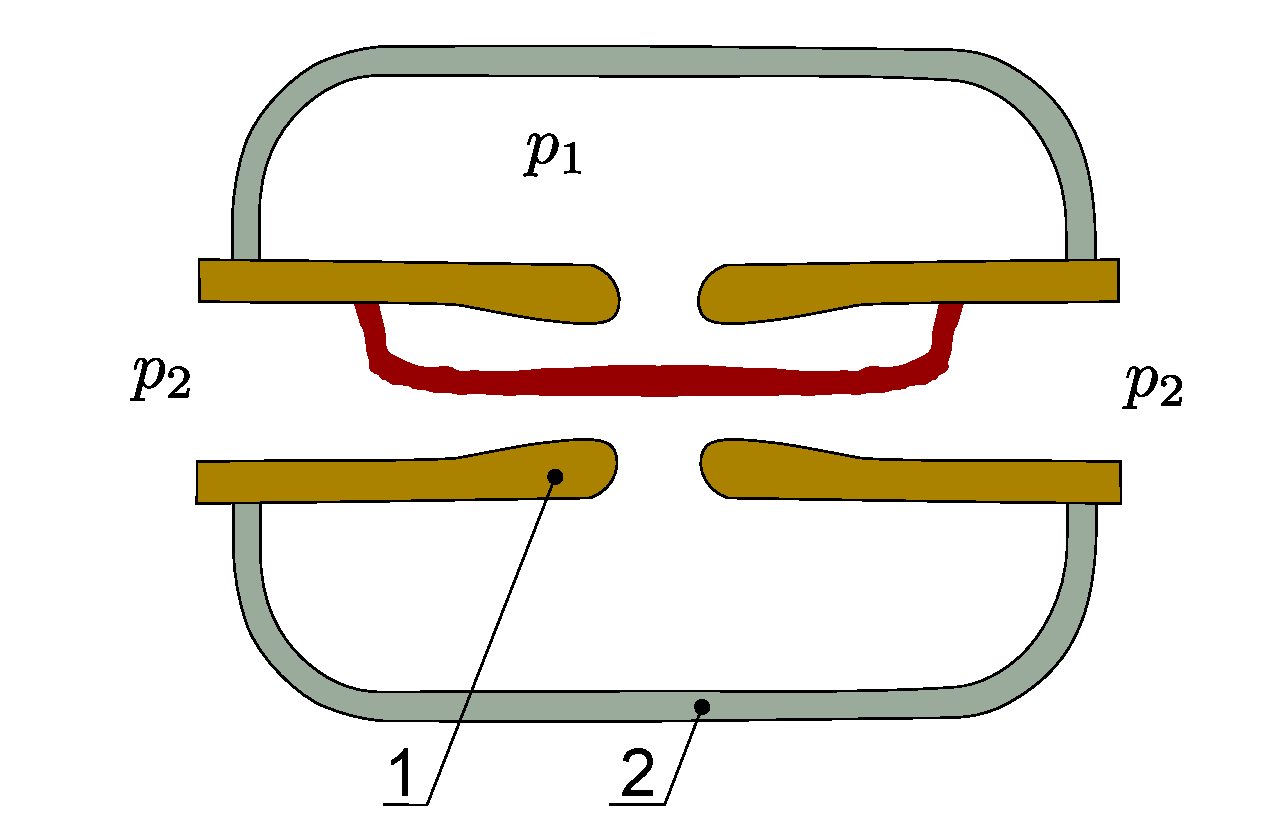
\includegraphics[width=0.6\linewidth]{Barta_Vostracky_Komora_dvoustrannym_proudenim.pdf}
        \caption[Schématické uspořádání zhášecí komory tlakovzdušného vypínače s dvoustranným
                 prouděním.]{Schématické uspořádání zhášecí komory tlakovzdušného vypínače s
                 dvoustranným prouděním.}
        \label{epr:fig_komora_2stran_proudenim}
      \end{figure}
              
      Na obrázcích je schématicky znázorněn oblouk, který je axiálně ofukován plynem z prostoru 
      zhášecí komory s tlakem $p_1$ přes zhášecí trysky dutinou kontaktů do výfuku, kde je nižší 
      tlak $p_2$.

      \subsubsection*{Legenda:}
        \begin{enumerate}[noitemsep]
         \item \emph{Zhášecí tryska}
         \item \emph{Tlaková izolační nádoba}
         \item \emph{Kontakt}
             \begin{itemize}
             %\item $D_t\cdots$ průměr zhášecí trysky
             %\item $D_s\cdots$ průměr styčné kružnice v zapnuté poloze kontaktů (měřený na 
             %      průměru $D_s$)
             %\item $z_k\cdots$ zdvih kontaktů (měřený na průměru $D_s$)
             %\item $x_1\cdots$ nejkratší vzdálenost kontaktů
             %\item $\alpha\cdots$ vrcholový úhel kontaktů
             \item $p_1\cdots$    tlak ve zhášecí komoře
             \item $p_2\cdots$    tlak ve výfukovém prostoru
             %\item $l_{ac}\cdots$ délka oblouku
             %\item $l_{a1}\cdots$ charakteristická délka oblouku
             \end{itemize}
        \end{enumerate}

    \subsubsection{Tři základní intervaly vypínacího pochodu}
      Vypínací pochod lze z hlediska zkoušení vypínačů rozdělit do tří základních intervalů:
      \begin{enumerate}[noitemsep]
        \item $t_s\cdots$ \textbf{Silnoproudý  interval}
        \item $t_i\cdots$ \textbf{Interakční interval}
        \item $t_d\cdots$ \textbf{Dielektrický interval}
      \end{enumerate}

      \begin{figure*}
        \centering
        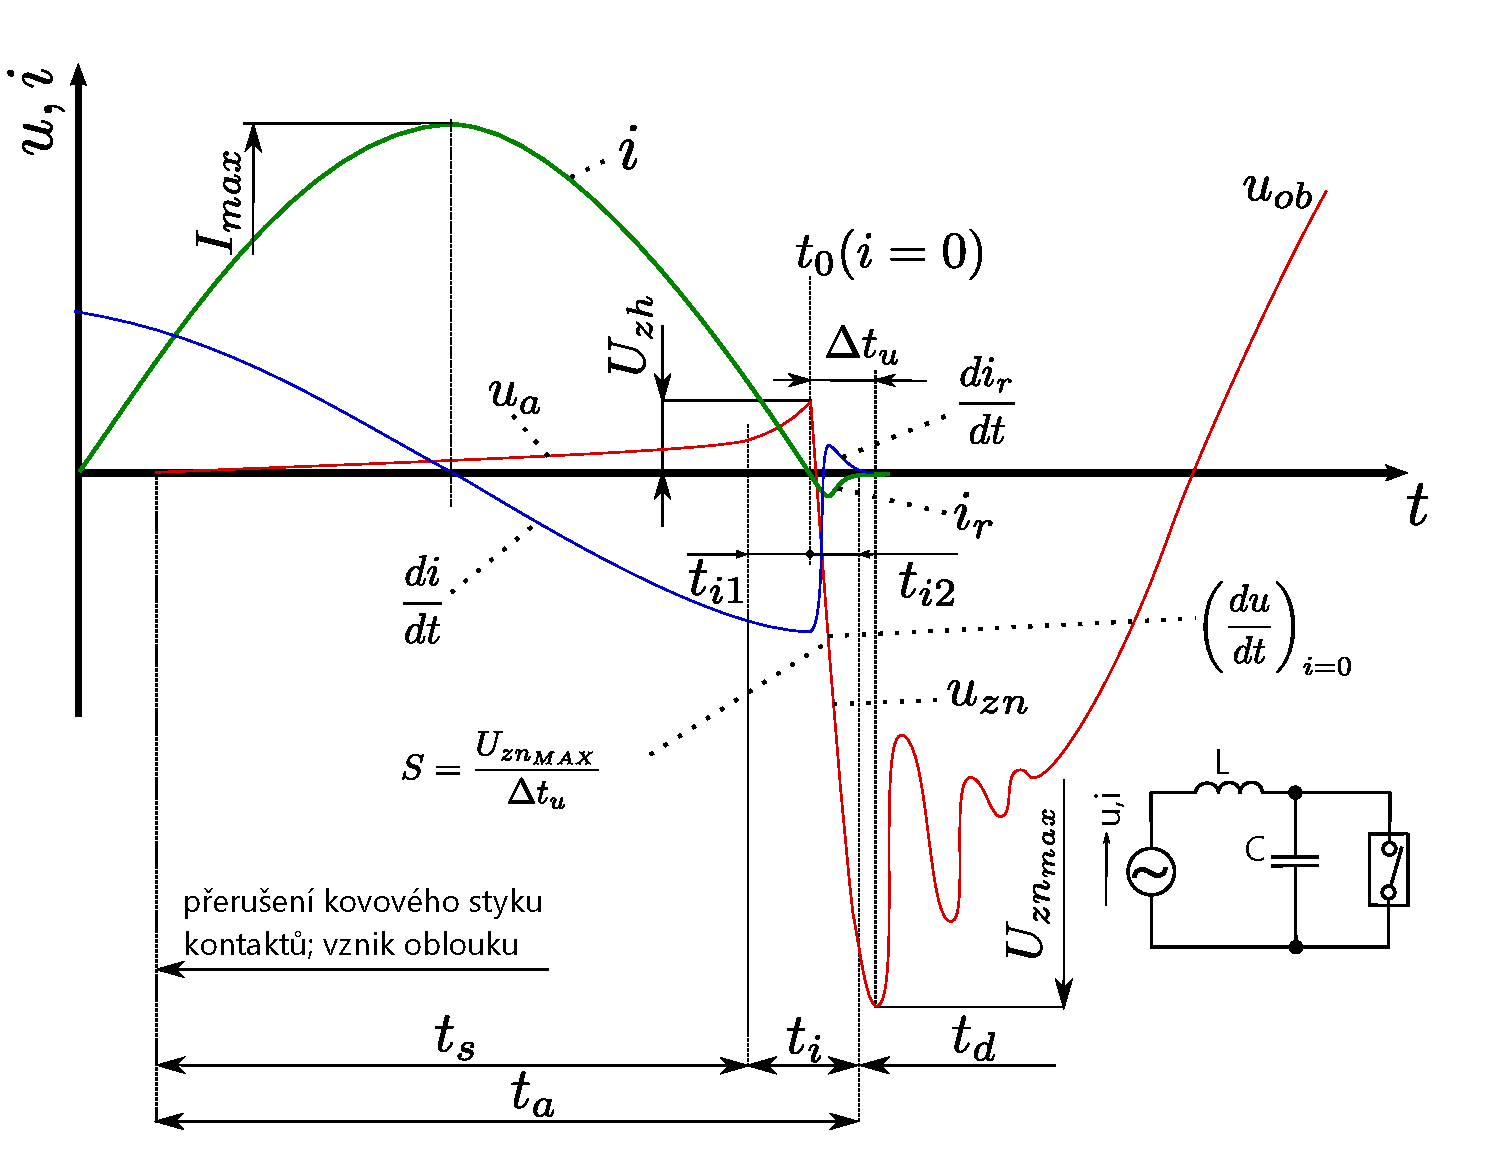
\includegraphics[width=0.8\textwidth]{Barta_Vostracky_Zakladni_intervaly_vypinaciho_pochodu.pdf}
        \caption[Základní intervaly vypínacího pochodu.]{Základní intervaly vypínacího pochodu.}
        \label{epr:fig_zakl_int_vyp_pochodu}
      \end{figure*}

      \begin{itemize}[noitemsep]
        \item $t_s\cdots$     silnoproudý interval
        \item $t_i\cdots$     interakční interval
          \begin{itemize}
            \item $t_{i1}\cdots$  interval výrazné změny obloukového napětí
            \item $t_{i2}\cdots$  interval zbytkového proudu
          \end{itemize}
        \item $t_d\cdots$    dielektrický interval
        \item $t_a\cdots$    doba hoření oblouku
        \item $\frac{di}{dt}\cdots$ derivace proudu podle času
        \item $i_r\cdots$    zbytkový proud
        \item $\frac{di_r}{dt}\cdots$ derivace zbytkového proudu podle času
        \item $u_a\cdots$    napětí oblouku
        \item $U_{zh}\cdots$ zhášecí amplituda napětí
        \item $U_{zn_{max}}\cdots$ maximální hodnota zotaveného napětí
        \item $u_{0b}\cdots$ obnovené napětí
        \item $S\cdots$      strmost zotaveného napětí (podle IEC)
        \item $\Delta t_u\cdots$ doba od průchodu proudu nulou do okamžiku protnutí tečny obalující
              křivku $u_{zn}$ v hodnotě $U_{zn_{max}}$
        \item $\left.\frac{du}{dt}\right\rvert_{i=0}\cdots$ okamžitá strmost
              zotaveného napětí v nulové hodnotě proudu
      \end{itemize}
      Charakteristické parametry vypínače v intervalech vypínacího pochodu:
      \begin{itemize}[noitemsep]
        \item $\mathbf{t_s}: i, I_{max}, u_a$
        \item $\mathbf{t_a}: \frac{di}{dt},i_r, \frac{du}{dt}, u_{zn}, U_{zn_{max}}$
        \item $\mathbf{t_d}: \frac{du}{dt}, S, U_{zn_{max}}$
      \end{itemize}

      Rozdělení vypínacího pochodu do těchto intervalů umožňuje snadněji specifikovat základní
      kritéria, kterým musí zhášecí komora vyhovovat při vypínání. Při vypínání střídavého proudu
      charakter proudění plynu závisí nejen na časově proměnlivém zdvihu kontaktů, druhu plynu a
      tlakových poměrech, ale i na předcházejícím proudu, přičemž všechny veličiny jsou vzájemně
      závislé. Hranice intervalů však lze určit jen přibližně, protože jsou závislé na kmitočtu
      proudu a na časové konstantě oblouku. Časová konstanta oblouku je proměn\-livá nejen s
      velikostí proudu, ale závisí i na uspořádání zhášecí komory.

  \subsection{Elektrický oblouk a jeho zhášení}
  \subsection{Zhášecí vlastnosti fluoridu sírového}
    Jak bylo uvedeno v předchozích kapitolách, ve zhášecí komoře vý\-ko\-no\-vých vypínačů po
    zhasnutí oblouku ještě zůstává po krátkou dobu mezi elektrodami zbytkové plazma, které obsahuje
    značný počet volných elektronů. Je-li toto množství kolem $10^{14}$ až $10^{15}$ elektronů v
    metru krychlovém, pak je splněna podmínka pro tvorbu \emph{elektronových lavin} nebo
    \emph{strimérů} a strmě stoupající zotavené napětí může způsobit jiskrový výboj, který přejde
    okamžitě v obloukový opětný zápal. Protože v plazmě oblouku je hustota elektronů závislá na její
    teplotě, nemá-li dojít k opětnému zápalu, musí plazmu dobře fungující vypínač rychle ochladit.
    Chladící  pochod je podmíněn vlastností plynu vyjádřenou \textbf{tepelnou vodivostí}
    $[\frac{W}{K\cdot m}]$,  kterou způsobují tyto dva dílčí jevy:
    \begin{itemize}
      \item Odvod kinetické energie plynu, který probíhá při vzájemných srážkách molekul 
            rozkmitaných tepelnou energií plynu,
      \item Disociace molekul, kdy při rozkladech molekul na základní atomy se při ne\-pru\-žných
            srážkách pohlcuje disociační energie a tím se kinetická energie molekul pře\-mě\-ňu\-je
            na potenciální energii atomů. Tato se odvádí difúzí do oblastí plynu s nízkou teplotou.
    \end{itemize}
    Disociace molekul nastává jen v úzkém teplotním intervalu charakterizovaném \textbf{disociační 
    teplotou} $\Theta_d$. Proto má křivka tepelné vodivosti plynu kolem teploty $\Theta_d$ značně 
    vyjádřené maximum.
    \begin{itemize}
      \item Plyn \ce{SF6}: \(\Theta_d = 2500 K\).
      \item Plyn \ce{N2} (vzduch): \(\Theta_d = 7500 K\).
    \end{itemize}
    Rozdílné teploty $\Theta_d$ jsou způsobeny tím, že disociační energie molekuly dusíku \ce{N2}
    je $14.5 eV$, zatímco síra $S$ disociuje z molekuly \ce{SF6} již při energii $10.4 eV$.
   
    \begin{figure}[ht!]
      \centering
      \subcaptionbox{Tepelné vodivosti dusíku (\ce{N2}) a fluoridu sírového (\ce{SF6}) \label{epr:fig_oblouk_vodivost}}
        {\luafigure[0.45]{char_vodivost_teplota_SF6_N2.pdf}}
      \subcaptionbox{Křivky rozdělení teplot oblouku v závislosti na poloměru oblouku v \ce{SF6}; 1 až 
                4 různé proudy oblouku \label{epr:fig_oblouk_trup}}
        {\luafigure[0.43]{rozdeleni_teplot_oblouku.pdf}}
      \caption{Základní charakteristiky oblouku hořícího v plynech \ce{SF6} a porovnání s dusíkem}
      \label{epr:fig_oblouk_char}
    \end{figure}
    Průběh křivek tepelných vodivostí různých plynů dovoluje současně odhadnout prostorové rozdělení
    teplot v elektrickém oblouku, neboť v místech s \emph{maximální tepelnou vodivostí je minimální
    teplotní spád (gradient)}. Proto se v křivkách znázorňující rozdělení teploty oblouku v
    závislosti na jeho poloměru objevují v okolí disociačních teplot pro dusík \ce{N2} a \ce{SF6}
    znatelné zlomy pro různé velikost proudů. Z těchto průběhů je také možné určit dvě zcela
    rozdílné oblasti oblouku:
    \begin{itemize}[noitemsep]
      \item \textbf{Trup oblouku}: velmi jasně zářící oblast s vysokými teplotami ležícími nad
            $\Theta_d$
      \item \textbf{Plášť oblouku}: difúzně svítivá část oblouku s teplotami dosahujícími maximálně
            $\Theta_d$
    \end{itemize}
    Důležitost disociační teploty $\Theta_d$ molekuly plynu zvlášť vyniká při sledování rychlosti
    zmenšování hustoty elektronů ve zbytkové plazmě oblouku, která je kritériem vzniku elektrického
    výboje mezi kontakty. Protože ve žhavém trupu je úbytek hustoty elektronů stokrát rychlejší než
    ve vnějším plášti oblouku, zaniká po nule proudu nejprve zářivý trup oblouku. \emph{Zotavené
    napětí} působí již jen na \emph{plášť oblouku}, v němž se hustota elektronů zmenšuje jen velmi
    zvolna. Protože kritickou veličinou pro elektrický výboj v plynném prostředí je hustota
    elektronů kolem $10^{14}/m^3$, bylo z kinetické teorie plynů odvozeno, že tento stav odpovídá
    přibližně teplotě kolem \textbf{3000 K}.
    
%---------------------------------------------------------------------------------------------------